\documentclass[11pt,a4paper]{article}
\usepackage[T1]{fontenc}
\usepackage{lmodern}
\usepackage[margin=2.3cm]{geometry}
\usepackage{amsmath,amssymb}
\usepackage{graphicx}
\usepackage{booktabs}
\usepackage{array}
\usepackage[hidelinks]{hyperref}
\usepackage{xcolor}
\graphicspath{{figures/}}
\newcommand{\code}[1]{\texttt{#1}}
\newcommand{\eminus}{e$^-$}
\newcommand{\gfit}{g_{\mathrm{fit}}}
\newcommand{\ncap}{n_{\mathrm{cap}}}
\newcommand{\nmax}{n_{\mathrm{max}}}
% a shaded box for worked examples
\newsavebox{\exbox}
\newenvironment{example}%
  {\par\smallskip\noindent\begin{lrbox}{\exbox}\begin{minipage}{0.96\linewidth}\small\textbf{Worked example.}\ }%
  {\end{minipage}\end{lrbox}\colorbox{black!6}{\usebox{\exbox}}\par\smallskip}
% a short "in words" note after an equation
\newcommand{\inwords}[1]{\par\noindent\textit{In words:} #1\par}

\title{The gain-vs-charge correction of skipper-CCD cluster energies:\\ what it does, exactly}
\author{\code{comm\_scripts}: \code{src/gain\_vs\_charge.py}, \code{bin/run\_WADERs --gain-correction}}
\date{22 October 2026}

\begin{document}
\maketitle

\begin{abstract}
The output amplifier of a skipper CCD does not turn charge into ADU with one constant gain: the
number of ADU that one more electron adds becomes slowly smaller as the charge in the pixel grows,
by about 3\,\% at 1000\,\eminus. panaSKImg converts every pixel with a single gain measured from
the 0\,\eminus{} and 1\,\eminus{} peaks, so X-ray clusters, whose pixels hold hundreds to thousands of
electrons, come out too low in energy, and by different amounts on different CCDs and images. This
note explains, step by step and with every formula spelled out, (1) why that happens and how large
the error is, (2) how the gain as a function of charge, $g(n)$, is measured from the images
themselves using the ``comb'' of electron peaks, (3) how $g(n)$ is modelled, (4) how it is used to
recompute each pixel and cluster energy, and (5) what it does to the Fe-55 (front-side) and Am-241
lines, including a comparison of the three model forms that can be chosen.
\end{abstract}

\tableofcontents

\section*{Symbols used in this note}
\begin{center}
\begin{tabular}{>{$}l<{$}p{12.2cm}}
\toprule
n & number of electrons in a pixel (an integer; ``charge'') \\
x & pixel value in ADU after pedestal subtraction (the average over all skips) \\
A(n) & the mean ADU of a pixel that holds $n$ electrons (the \emph{response}); $A(0)=0$ \\
g(n) & the \emph{local gain} $dA/dn$: how many ADU one more electron adds at charge $n$ [ADU/\eminus] \\
g(0) & local gain at low charge (in practice: at the first measured point, $\approx 25$\,\eminus) \\
g_0 & starting estimate of the low-charge gain (from \code{autoconfig\_panaSKImg.py}), used to define charge bins \\
\gfit & the single gain panaSKImg used for an image and CCD (stored in the cluster file) \\
\varepsilon & 3.74\,eV, the energy per electron used by panaSKImg \\
E_{\mathrm{pix}},\ E & energy of one pixel, energy of a cluster (sum of its pixels) \\
R & comb visibility (Sec.~\ref{sec:R}): 1 = perfect comb, $\approx 0$ = no comb \\
N & number of pixels in a sample \\
\nmax & highest charge up to which $g(n)$ is measured \\
\ncap & $3\,\nmax$: above this charge $g$ is held constant \\
\Delta(n) & nonlinearity: apparent minus true number of electrons (Sec.~\ref{sec:delta}) \\
\bottomrule
\end{tabular}
\end{center}

%======================================================================
\section{The problem}
%======================================================================
\subsection{How a pixel value relates to its charge}
A skipper CCD measures the charge of each pixel many times (500 skips for Image 5) and averages the
measurements, so the read noise in the average is small (here 0.14--0.22\,\eminus). After the
pedestal (the value of an empty pixel) is subtracted, the value of a pixel holding $n$ electrons is
\begin{equation}
x = A(n) + \epsilon, \qquad A(n) = \int_0^n g(m)\,dm .
\label{eq:A}
\end{equation}
\inwords{the pixel value $x$ is the amplifier's mean response $A(n)$ to $n$ electrons plus a small
random read-noise term $\epsilon$. The response is built up electron by electron: the first electron
adds $g(0)$ ADU, an electron added when the pixel already holds $m$ electrons adds $g(m)$ ADU, and
$A(n)$ is the sum (integral) of all these increments. $g(n)$ is the slope of $A(n)$, which is why
it is called the \emph{local} gain.}

If the amplifier were perfectly linear, $g$ would be a constant and $A(n) = g\,n$: every electron
would add the same number of ADU. In reality $g(n)$ decreases slowly with $n$ (and on a few CCDs it
first increases a little, Sec.~\ref{sec:forms}).

\begin{example}
DM09 EXT4 (curve from three Image 5s, Sec.~\ref{sec:fe55}): $g(0)=1.2667$, $g(100)=1.2643$,
$g(500)=1.2475$ and $g(1000)=1.2282$\,ADU/\eminus. The response is $A(100)=126.6$,
$A(500)=629.2$ and $A(1000)=1247.5$\,ADU. A linear amplifier with gain 1.2667 would give
$1266.7$\,ADU for 1000 electrons, 19.2\,ADU (1.5\,\%) more.
\end{example}

\subsection{What panaSKImg does with the pixel values}
panaSKImg fits the electron peaks at low charge (in \code{run\_WADERs}: the 0\,\eminus{} and 1\,\eminus{}
peaks, or a fit of several peaks) and obtains one gain $\gfit$ per CCD and image. It converts every
pixel to energy as if the amplifier were linear with that gain:
\begin{equation}
E_{\mathrm{pix}} = \varepsilon\,\frac{x}{\gfit}, \qquad \varepsilon = 3.74\ \mathrm{eV}/e^- .
\label{eq:epix}
\end{equation}
\inwords{dividing the ADU by the gain gives a number of electrons, and multiplying by 3.74\,eV per
electron gives an energy. The energy of a cluster is the sum of its pixel energies,
$E = \sum_j E_{\mathrm{pix},j}$.}

\subsection{How large the error is, and what it depends on}
\label{sec:bias}
A cluster whose pixels hold $n_1, n_2, \dots$ electrons has the true energy
$E_{\mathrm{true}} = \varepsilon \sum_j n_j$. panaSKImg reports, from Eqs.~\ref{eq:A} and~\ref{eq:epix}
(ignoring the noise, which averages out over many clusters),
\begin{equation}
E = \varepsilon \sum_j \frac{A(n_j)}{\gfit} .
\label{eq:Erep}
\end{equation}
To see the size of the error, approximate the gain by a straight line, $g(n) = a + b\,n$, with $a$
the low-charge gain and $b<0$ its slope. Integrating (Eq.~\ref{eq:A}) gives
$A(n) = a\,n + \tfrac{1}{2}b\,n^2$. Inserting this in Eq.~\ref{eq:Erep} and dividing by $E_{\mathrm{true}}$:
\begin{equation}
\frac{E}{E_{\mathrm{true}}} = \frac{\sum_j \big(a\,n_j + \tfrac12 b\,n_j^2\big)}{\gfit\sum_j n_j}
= \frac{a}{\gfit} + \frac{b}{2\gfit}\,\frac{\sum_j n_j^2}{\sum_j n_j},
\end{equation}
so the relative error is
\begin{equation}
\frac{E}{E_{\mathrm{true}}} - 1 \;=\; \underbrace{\left(\frac{a}{\gfit} - 1\right)}_{\text{(i) calibration}}
\;+\; \underbrace{\frac{b}{2\gfit}\,\langle n\rangle_w}_{\text{(ii) nonlinearity}},
\qquad
\langle n\rangle_w \equiv \frac{\sum_j n_j^2}{\sum_j n_j} .
\label{eq:bias}
\end{equation}
\inwords{the error has two independent parts.
(i) The \emph{calibration} term: if panaSKImg's gain $\gfit$ is not equal to the true low-charge gain
$a$, every pixel is off by the same fraction. This term differs from image to image, because each
image has its own fit. (ii) The \emph{nonlinearity} term: because $b<0$, bright pixels give too few ADU.
How much depends on $\langle n\rangle_w$, the average pixel charge \emph{weighted by charge}: the typical
charge of the pixel that a given electron of the cluster sits in. A compact cluster (front side,
little diffusion) puts its electrons in a few bright pixels, has a large $\langle n\rangle_w$, and is
shifted more than a diffuse cluster of the same energy.}

\begin{example}
A cluster of 1580 electrons (5.909\,keV) in six pixels with 900, 400, 150, 80, 30 and 20\,\eminus{}
has $\langle n\rangle_w = (900^2 + 400^2 + \dots)/1580 = 633$\,\eminus. On DM09 EXT4 a straight line
through the measured gains has $a = 1.2677$ and $b = -3.79\times10^{-5}$\,ADU/\eminus$^2$, and the
image's fitted gain is $\gfit = 1.2759$. Eq.~\ref{eq:bias} gives (i) $1.2677/1.2759 - 1 = -0.64\,\%$ and
(ii) $-3.79\times10^{-5}\times 633/(2\times1.2759) = -0.94\,\%$: together $-1.58\,\%$. Computing
Eq.~\ref{eq:Erep} exactly with the measured curve gives 5.813\,keV, i.e.\ $-1.62\,\%$. For the real
front-side Fe-55 K$\alpha$ clusters of DM09/DM10, $\langle n\rangle_w$ is 570--1480\,\eminus{} (10th to 90th
percentile, median 1050), and their brightest pixel holds a median of 1250\,\eminus{} (90\,\% below 1520).
\end{example}

The general form of Eq.~\ref{eq:bias}, without assuming a straight line, is given in
Eq.~\ref{eq:biasgen} below. The correction described in this note removes \emph{both} terms, by
converting each pixel with the measured $A(n)$ instead of $\gfit$.

\subsection{The nonlinearity curve}
\label{sec:delta}
A common way to display the nonlinearity is the charge a pixel \emph{appears} to hold, minus the
charge it really holds, against the apparent charge. In this note and in the outputs of the code,
the apparent charge is computed with the curve's own low-charge gain $g(0)$:
\begin{equation}
n_{\mathrm{meas}}(n) = \frac{A(n)}{g(0)}, \qquad
\Delta(n) = n_{\mathrm{meas}}(n) - n .
\label{eq:delta}
\end{equation}
\inwords{$n_{\mathrm{meas}}$ is the number of electrons one would infer from the pixel value if one
assumed the gain stays at its low-charge value; $\Delta$ is how many electrons that inference is off.
Because the reference is $g(0)$, the calibration term of Eq.~\ref{eq:bias} is absent and $\Delta$
shows only the nonlinearity: it starts at $\Delta=0$ and bends down where the gain falls.}

For a straight line, $g(0)=a$ and $A(n)/a = n + \frac{b}{2a}n^2$, so
\begin{equation}
\Delta(n) = \frac{b}{2a}\,n^2 \qquad (\text{straight-line gain}),
\label{eq:parab}
\end{equation}
an exact parabola. A gain that falls by 3\,\% at 1000\,\eminus{} ($b/a = -3\times10^{-5}$) gives
$\Delta(1000) = -15$\,\eminus. In the plots a quadratic $c_2 x^2 + c_1 x$ through the origin
($x = n_{\mathrm{meas}}$) is fitted as a compact summary: $c_2 \approx b/2a$, and $c_1 \neq 0$ signals
that the curve is not a parabola (for example on a CCD whose gain first rises, where $\Delta$ goes
\emph{up}).

\paragraph{The general error formula.} With $\Delta$ the error of Eq.~\ref{eq:bias} can be written for
any $g(n)$: since $A(n_j) = g(0)\,[n_j + \Delta(n_j)]$,
\begin{equation}
\frac{E}{E_{\mathrm{true}}} = \frac{g(0)}{\gfit}\left(1 + \frac{\sum_j \Delta(n_j)}{\sum_j n_j}\right).
\label{eq:biasgen}
\end{equation}
\inwords{the first factor is the calibration error, the second the nonlinearity: the electrons
``lost'' by all pixels of the cluster, as a fraction of the cluster's electrons.}

\paragraph{With panaSKImg's gain as the reference.} If $\gfit$ is used in Eq.~\ref{eq:delta} instead of
$g(0)$, a linear term $(a/\gfit - 1)\,n$ is added: the curve then rises at first whenever $\gfit < a$,
and only bends down at high charge. That mixes the calibration error into the curve, so the code always
uses $g(0)$.

\begin{figure}[t]
\centering
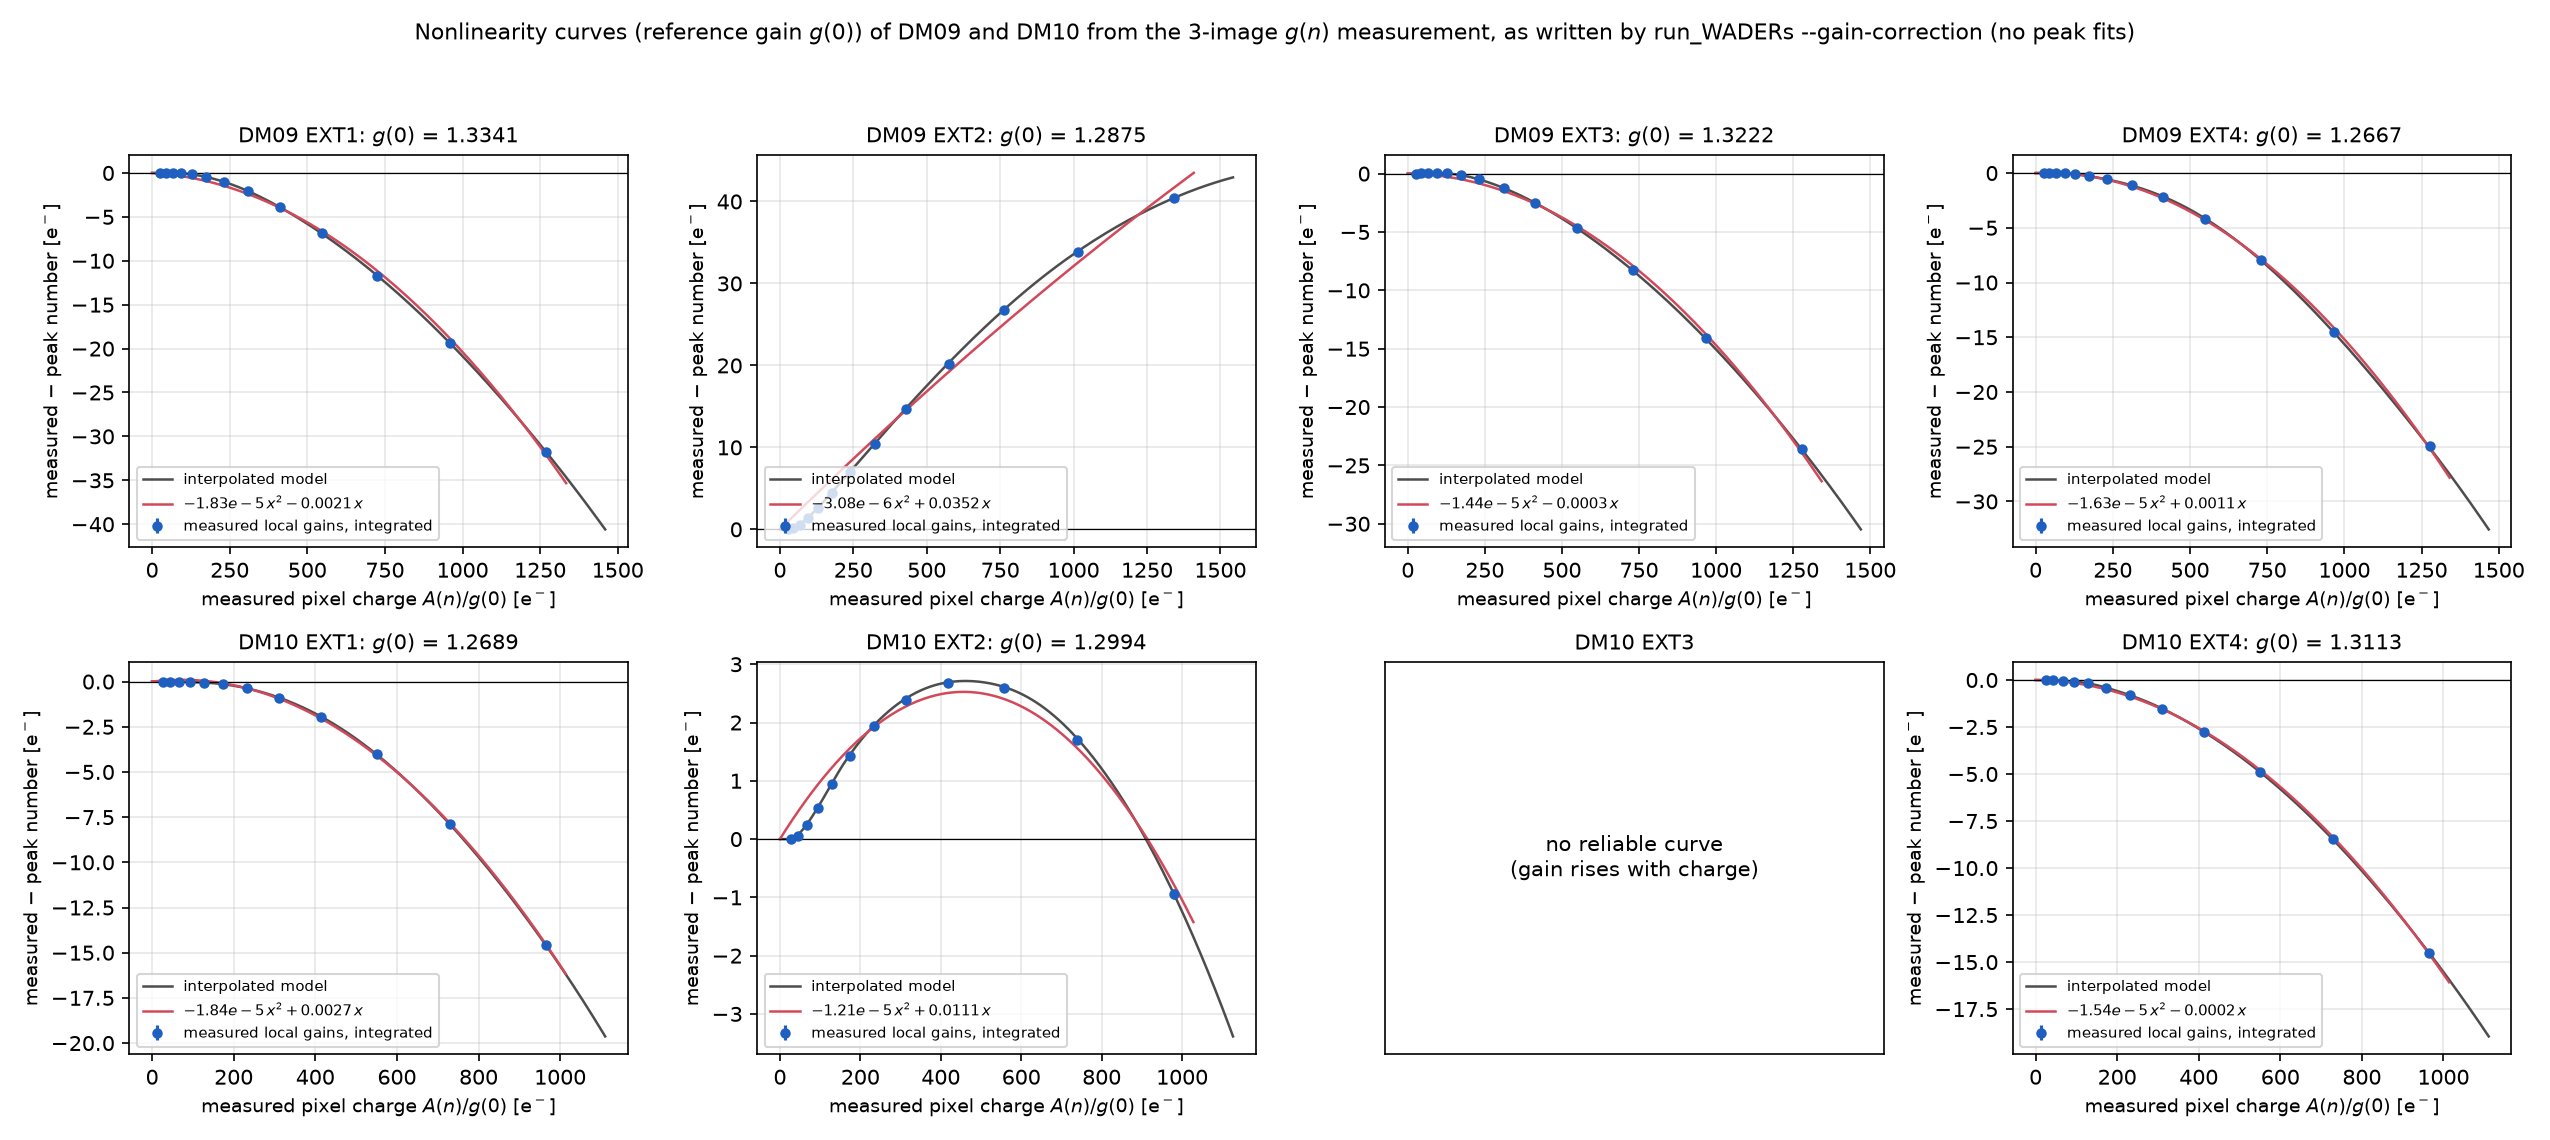
\includegraphics[width=\textwidth]{nonlinearity.png}
\caption{Nonlinearity curves $\Delta$ (Eq.~\ref{eq:delta}, reference $g(0)$) of the CCDs of DM09 and DM10,
from the 3-image $g(n)$ measurement. Points: the measured local gains, integrated (Sec.~\ref{sec:deltapts});
line: the interpolated model; red: quadratic fit. Typical values are $\Delta(1000) = -15$ to $-20$\,\eminus{}
($c_2 = -1.4$ to $-1.8\times10^{-5}$). DM09 EXT2 and DM10 EXT2 are the CCDs whose gain first rises with
charge (Fig.~\ref{fig:forms}), so $\Delta$ goes up; DM10 EXT3 has no reliable curve. \code{run\_WADERs
--gain-correction} writes this plot for every curve (\code{gain\_vs\_charge/*\_nonlinearity.png}).}
\label{fig:nonlin}
\end{figure}

%======================================================================
\section{Measuring $g(n)$ from the electron comb}
\label{sec:measure}
%======================================================================
\subsection{The idea}
Because the read noise (0.14--0.22\,\eminus) is much smaller than one electron, the pixel values do
not form a smooth distribution but a \emph{comb}: a narrow peak (``tooth'') at $A(n)$ for every
integer $n$ (Fig.~\ref{fig:comb}, left). The comb is not only present at low charge. X-ray clusters,
particle tracks and the halo around bright events contain pixels with every charge up to thousands
of electrons, and there the teeth are still there. The distance between neighbouring teeth is
\begin{equation}
A(n+1) - A(n) = \int_n^{n+1} g(m)\,dm \approx g\!\left(n + \tfrac12\right),
\end{equation}
\inwords{the spacing of the comb around $n$ electrons \emph{is} the local gain at $n$.}
So $g(n)$ can be read off the images directly, at every charge where enough pixels exist; no
radioactive source and no peak-by-peak fit are needed. The steps below are those of
\code{gain\_vs\_charge.measure}.

\subsection{Step 1: pixels and pedestal}
For every CCD (extension) the active pixels are taken from the image, skipping the first 3 rows
(they carry a readout transient). The pedestal of each row is the median of that row's overscan
pixels, which are empty by construction (for windowed readouts without overscan, the median of the
active row is used: it sits on the 0\,\eminus{} peak because most pixels are empty):
\begin{equation}
x_{rc} = \mathrm{raw}_{rc} - \operatorname{median}_{c' \in \text{overscan}} \mathrm{raw}_{rc'} .
\end{equation}
\inwords{subtract from each pixel ($r$ = row, $c$ = column) the typical value of an empty pixel in the
same row.} A starting value $g_0$ of the low-charge gain comes from \code{autoconfig\_panaSKImg.py}
(the comb spacing of the low-charge pixels); it is only used to define the charge bins and the search
range below.

\subsection{Step 2: aligning the rows}
The median of $\sim$150 overscan pixels is not perfectly accurate: from row to row the pedestal can be
off by a fraction of an electron, which shifts the whole comb of that row and blurs the comb of the
image. Each row $r$ is therefore shifted so that its teeth sit at integer multiples of $g_0$:
\begin{equation}
\phi_r = \arg \Big\langle e^{2\pi i\,x/g_0} \Big\rangle_{\text{row } r,\ |x|<3g_0}, \qquad
x \;\to\; x - \frac{g_0\,\phi_r}{2\pi} .
\label{eq:align}
\end{equation}
\inwords{each pixel value is turned into an angle, $2\pi x/g_0$, i.e.\ its position within a tooth
expressed as a point on a circle (one full turn per electron). Averaging the unit vectors
$e^{2\pi i x/g_0}$ of the low-charge pixels of the row gives a vector whose angle $\phi_r$ is the mean
position of that row's teeth within a tooth (a ``circular mean'', which handles the wrap-around at
$\pm$half a tooth correctly). Shifting the row by $\phi_r/2\pi$ of a tooth moves its teeth back to
the integers.} Whole-electron offsets are not corrected (and do not matter: they do not change the
spacing).

\subsection{Step 3: keeping only clean rows}
After a very bright event the readout is disturbed for a while and the comb of the following rows is
blurred. Rows are grouped in blocks of 25, and for each block $b$ the comb \emph{visibility} of its
pixels with 0.5 to 30\,\eminus{} is computed:
\begin{equation}
V_b = \Big| \Big\langle e^{2\pi i\,x/g_0} \Big\rangle_{\text{block } b,\ 0.5 g_0 < x < 30 g_0} \Big| .
\label{eq:vis}
\end{equation}
\inwords{the same unit vectors as in Eq.~\ref{eq:align}, but now we look at the \emph{length} of their
average. If every pixel sits exactly on a tooth, all vectors point the same way and the length is 1.
If the comb is washed out, the vectors point in all directions and their average is close to 0.
In between, the length measures how sharp the comb is.} Only blocks with $V_b \ge 0.6\,\max_b V_b$
(and at least 300 such pixels) are used.

\subsection{Step 4: the local spacing in a charge bin}
\label{sec:R}
The clean pixels are split into charge bins with edges
\[ 20,\ 35,\ 55,\ 80,\ 110,\ 150,\ 200,\ 270,\ 360,\ 480,\ 640,\ 850,\ 1130,\ 1500,\ 2000,\ 2700,\ \dots\ e^- \]
(a pixel belongs to bin $[n_{lo}, n_{hi}]$ if $n_{lo}\,g_0 < x < n_{hi}\,g_0$). The bins are about 30\,\%
wide: wide enough to contain many pixels, narrow enough that $g$ changes little inside. In every bin
with at least 400 pixels (at most $3\times10^5$ are used, chosen at random), the spacing is found as the
trial period $g$ that makes the teeth line up best:
\begin{equation}
R(g) = \Big| \frac{1}{N} \sum_{k=1}^{N} e^{2\pi i\,x_k/g} \Big|, \qquad
\hat g = \arg\max_{g} R(g), \quad 0.85\,g_0 \le g \le 1.10\,g_0 .
\label{eq:R}
\end{equation}
\inwords{for a trial period $g$, every pixel's position within a tooth of period $g$ is turned into a
unit vector, and $R(g)$ is the length of their average, exactly as in Eq.~\ref{eq:vis}. Only when $g$
equals the true spacing do the pixels of all the different teeth in the bin land at the same position
in their tooth, so that the vectors line up and $R$ is large. The best period $\hat g$ is the local
gain of that bin.} The search is done on 351 trial values, then on 121 finer values around the best.
This is the Rayleigh test for periodicity, also called a periodogram.

Fig.~\ref{fig:comb} (right) shows what Eq.~\ref{eq:R} does: all pixels of a bin are folded onto one
tooth, $\mathrm{frac}(x/g)$. Folded with the low-charge gain $g_0$, the teeth of a high-charge bin fall
at different positions and the folded distribution is flat ($R \approx 0$); folded with the correct
local spacing they coincide and form a peak. The measured value is assigned to the charge
$n = \sqrt{n_{lo}\,n_{hi}}$ (the geometric centre of the bin; the bins are narrow enough that the exact
choice matters little).

\begin{figure}[t]
\centering
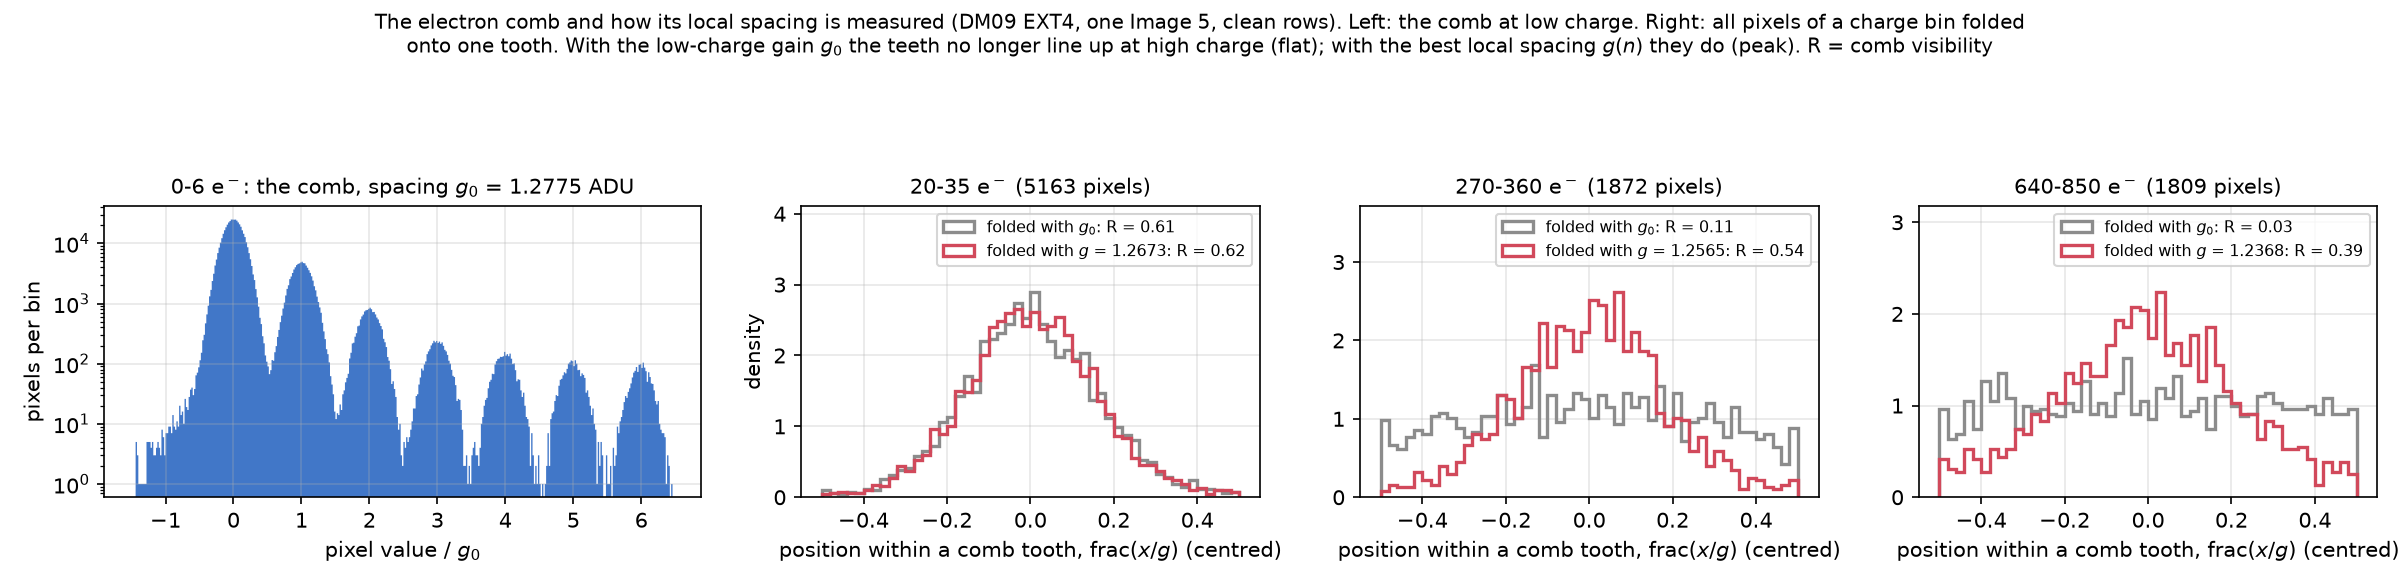
\includegraphics[width=\textwidth]{comb.png}
\caption{Left: the comb at low charge (log scale). Right: the pixels of three charge bins folded onto
one tooth with the low-charge gain $g_0$ (grey) and with the best local spacing $\hat g$ (red), centred
on their mean position. At 640--850\,\eminus{} the teeth are invisible with $g_0$ ($R=0.03$) but clear
with $\hat g = 0.968\,g_0$ ($R = 0.39$): the local gain there is 3.2\,\% lower than at low charge.}
\label{fig:comb}
\end{figure}

\subsection{Step 5: is the comb really there, and how precise is $\hat g$?}
\paragraph{Significance.} If the pixels have no comb at all (random positions within a tooth), the
average of $N$ random unit vectors still has some length by chance. Its square, $N R^2$, then follows an
exponential distribution with mean 1, so the probability to find $R > r$ by chance is
\begin{equation}
P(R > r) = e^{-N r^2} .
\label{eq:pnoise}
\end{equation}
\inwords{a random pile of pixels gives $R \approx 1/\sqrt N$; a value much larger than that is a real
comb.} A bin counts as measured if $R > 4/\sqrt N$, i.e.\ $N R^2 > 16$, which happens by chance with
probability $e^{-16} \approx 10^{-7}$. The scan through the bins stops after two consecutive bins fail.

\paragraph{Uncertainty.} Changing the trial period by $\delta g$ rotates the vector of a pixel with
$n$ electrons by an angle proportional to its distance from the bin centre, $\approx 2\pi(n - n_c)\,
\delta g/g$. Finding $\hat g$ is therefore like fitting the slope of a straight line (angle against
$n - n_c$) through $N$ points spread uniformly over the bin width $\Delta n = n_{hi} - n_{lo}$
(standard deviation $\Delta n/\sqrt{12}$), each with an angular scatter that grows as the comb gets
less sharp (roughly $1/R$). The usual straight-line formula then gives
\begin{equation}
\sigma_{\hat g} = \frac{g}{2\pi\,(\Delta n/\sqrt{12})\,R\,\sqrt N} .
\label{eq:sigma}
\end{equation}
\inwords{the local gain is more precise when there are more pixels ($\sqrt N$), when the comb is
sharper ($R$), and when the bin is wider (more lever arm, $\Delta n$).}

\begin{example}
DM09 EXT4, three images, bin 640--850\,\eminus: $N = 5490$ pixels, $R = 0.394$, $\hat g = 1.2365$
ADU/\eminus. Eq.~\ref{eq:sigma}: $\sigma = 1.2365 / (2\pi \times (210/\sqrt{12}) \times 0.394 \times
\sqrt{5490}) = 1.1\times10^{-4}$\,ADU/\eminus{} (0.009\,\%). The significance is
$N R^2 = 852 \gg 16$.
\end{example}

\paragraph{Why the measured range ends near 1000--1500\,\eminus.} Two things limit it. First, there
are fewer pixels at high charge. Second, inside one bin the gain itself changes, so the teeth are not
exactly periodic. With a straight-line gain the teeth at the edge of a bin, half a bin width
($\Delta n/2$) from the centre, are displaced from a periodic comb by
\begin{equation}
\delta\phi \approx 2\pi\,\frac{|b|}{2g}\left(\frac{\Delta n}{2}\right)^2
\end{equation}
of a full turn. For DM09 EXT4 in the bin 640--850\,\eminus{} this is $2\pi \times (3.79\times10^{-5}/2/1.2365)
\times 105^2 = 1.06$\,rad, a sixth of a tooth: the comb visibility drops, and in the next, wider bins it
disappears. The measured range ends at $\nmax$ = 1130--1500\,\eminus{} on Image 5 and 480--1130\,\eminus{}
on the AMT Image 8s. More images do not extend it (Sec.~\ref{sec:fe55}), because this is a limit of the
method, not of statistics.

\subsection{Step 6: several images of the same CCD}
\label{sec:multi}
Images of the same module can be combined. Each image $i$ is folded on its own and the comb
\emph{powers} are added:
\begin{equation}
R(g) = \sqrt{ \frac{\sum_i |S_i(g)|^2}{\sum_i N_i^2} }, \qquad S_i(g) = \sum_{k \in \text{image } i} e^{2\pi i\,x_k/g},
\label{eq:Rmulti}
\end{equation}
\inwords{$S_i$ is the sum of the unit vectors of image $i$ (Eq.~\ref{eq:R} without dividing by $N$);
its length $|S_i|$ measures how well image $i$'s teeth line up with period $g$, and its direction
says where those teeth sit. Squaring the length throws the direction away, so the images are added
regardless of where each image's teeth are. For one image this is identical to Eq.~\ref{eq:R}.}
The significance threshold becomes $R > 4\sqrt{\sum_i N_i/\sum_i N_i^2}$: four times the value that
pure noise gives on average (it reduces to $4/\sqrt N$ for one image).

\paragraph{Why the pixels must not simply be pooled.} Putting all pixels of all images into one sum
would require the teeth of every image to sit at the same place. They do not: the teeth of image $i$
are at $A_i(n)$, and if two images differ in gain by a small fraction $\delta g/g$, their teeth at
charge $n$ are displaced by about $n\,\delta g/g$ electrons from each other, i.e.\ by the angle
$2\pi\,n\,\delta g/g$. At $n = 850$ a difference of 0.1\,\% (typical between exposures) is
$2\pi \times 0.85$, almost a whole tooth: the teeth of one image fill the gaps of the other and the
pooled comb disappears. (The code before 22 October 2026 pooled the pixels; for 2--3 images its measured
range was then 850--1130 instead of 1130--1500\,\eminus.)

\subsection{Step 7: when a curve is trusted}
A curve is used only if (a) at least 4 bins are measured, (b) $\nmax \ge 400$\,\eminus, and (c) the slope
of a straight line through the points is not positive. Otherwise that CCD is left uncorrected. In the
data shown here this happens for a noisy image (DM10 image 0: noise 0.40--0.56\,\eminus{} instead of 0.21,
comb visible in only 50 of 475 rows) and for DM10 EXT3, whose gain rises by 1--1.6\,\% per 1000\,\eminus{}
in every image. Rule (c) treats a rising gain as a sign that something is wrong; it may be too strict
for CCDs like DM10 EXT3, but nothing is changed without a reason.

\subsection{The nonlinearity points}
\label{sec:deltapts}
The points of Fig.~\ref{fig:nonlin} come straight from the measured local gains $\hat g_k$ at the bin
centres $n_k$: $A$ is integrated with the trapezoid rule, holding $g$ at the first point below it,
\begin{equation}
A(n_1) = \hat g_1\,n_1, \qquad
A(n_k) = A(n_{k-1}) + \tfrac12\,(\hat g_{k-1} + \hat g_k)\,(n_k - n_{k-1}),
\end{equation}
and then $\Delta_k = A(n_k)/g(0) - n_k$ (Eq.~\ref{eq:delta}). The error of $A(n_k)$ adds the errors of
all bins below it in quadrature, each multiplied by its bin width.

%======================================================================
\section{Models of $g(n)$}
\label{sec:forms}
%======================================================================
The measured points $(n_k, \hat g_k \pm \sigma_k)$ are turned into a continuous curve in one of three
forms, chosen with \code{--model} in \code{gain\_vs\_charge.py} and \code{--gain-model} in
\code{run\_WADERs}.

\paragraph{interpolated (default).} A smooth curve that goes exactly through every measured point:
monotone piecewise-cubic Hermite interpolation (PCHIP). Between two neighbouring points the curve is a
cubic polynomial fixed by the values at the two points and by a slope at each point. The slope at a
point is a weighted harmonic mean of the slopes of the two straight segments next to it, and it is set
to zero where the data have a local maximum or minimum. This makes the curve rise or fall
monotonically between points, so it never overshoots or wiggles where the data do not. Below the first
point ($\approx 26$\,\eminus) $g$ is held at the first point's value; between the last point and $\nmax$
it continues with the slope $s$ of a straight line through the last 4 points.
\inwords{use the measurement as it is, without assuming a shape.}

\paragraph{broken.} Two straight lines that meet at a knot $n_k$:
\begin{equation}
g(n) = a + b_1 \min(n, n_k) + b_2 \max(n - n_k, 0) .
\end{equation}
\inwords{below the knot the gain changes with slope $b_1$, above it with slope $b_2$; the four numbers
$a, b_1, b_2, n_k$ are fitted by weighted least squares (minimising $\sum_k (g(n_k) - \hat g_k)^2/
\sigma_k^2$, starting from knots at 80--600\,\eminus{} and keeping the best).}

\paragraph{linear.} $g(n) = a + b\,n$, an unweighted straight-line fit through the points: the original
model, kept for comparison.

\paragraph{Above the measured range.} Beyond $\nmax$ there are no measurements. For every form the
curve continues as a straight line with its slope at $\nmax$ up to $\ncap = 3\,\nmax$, and is held
constant above:
\begin{equation}
g(n) = g\big(\min(n, \ncap)\big) .
\end{equation}
\inwords{assume the gain keeps falling at the same rate for a while, but not forever.}
The factor 3 was chosen on the AMT Am-241 data with the linear form: unlimited extrapolation
overcorrected CCDs with very compact clusters, while no extrapolation undercorrected the 59.5\,keV
line. It is a choice, not a measurement, and it matters only for pixels above $\nmax$ (Sec.~\ref{sec:am}).

\begin{example}
DM09 EXT4: $\nmax = 1500$\,\eminus, $\ncap = 4500$\,\eminus. The interpolated curve has
$g(1500) = 1.2162$ and an end slope $s = -2.98\times10^{-5}$\,ADU/\eminus$^2$, so $g(3000) = 1.1716$,
$g(4500) = 1.1269$, and $g = 1.1269$ for all higher charges.
\end{example}

\begin{figure}[t]
\centering
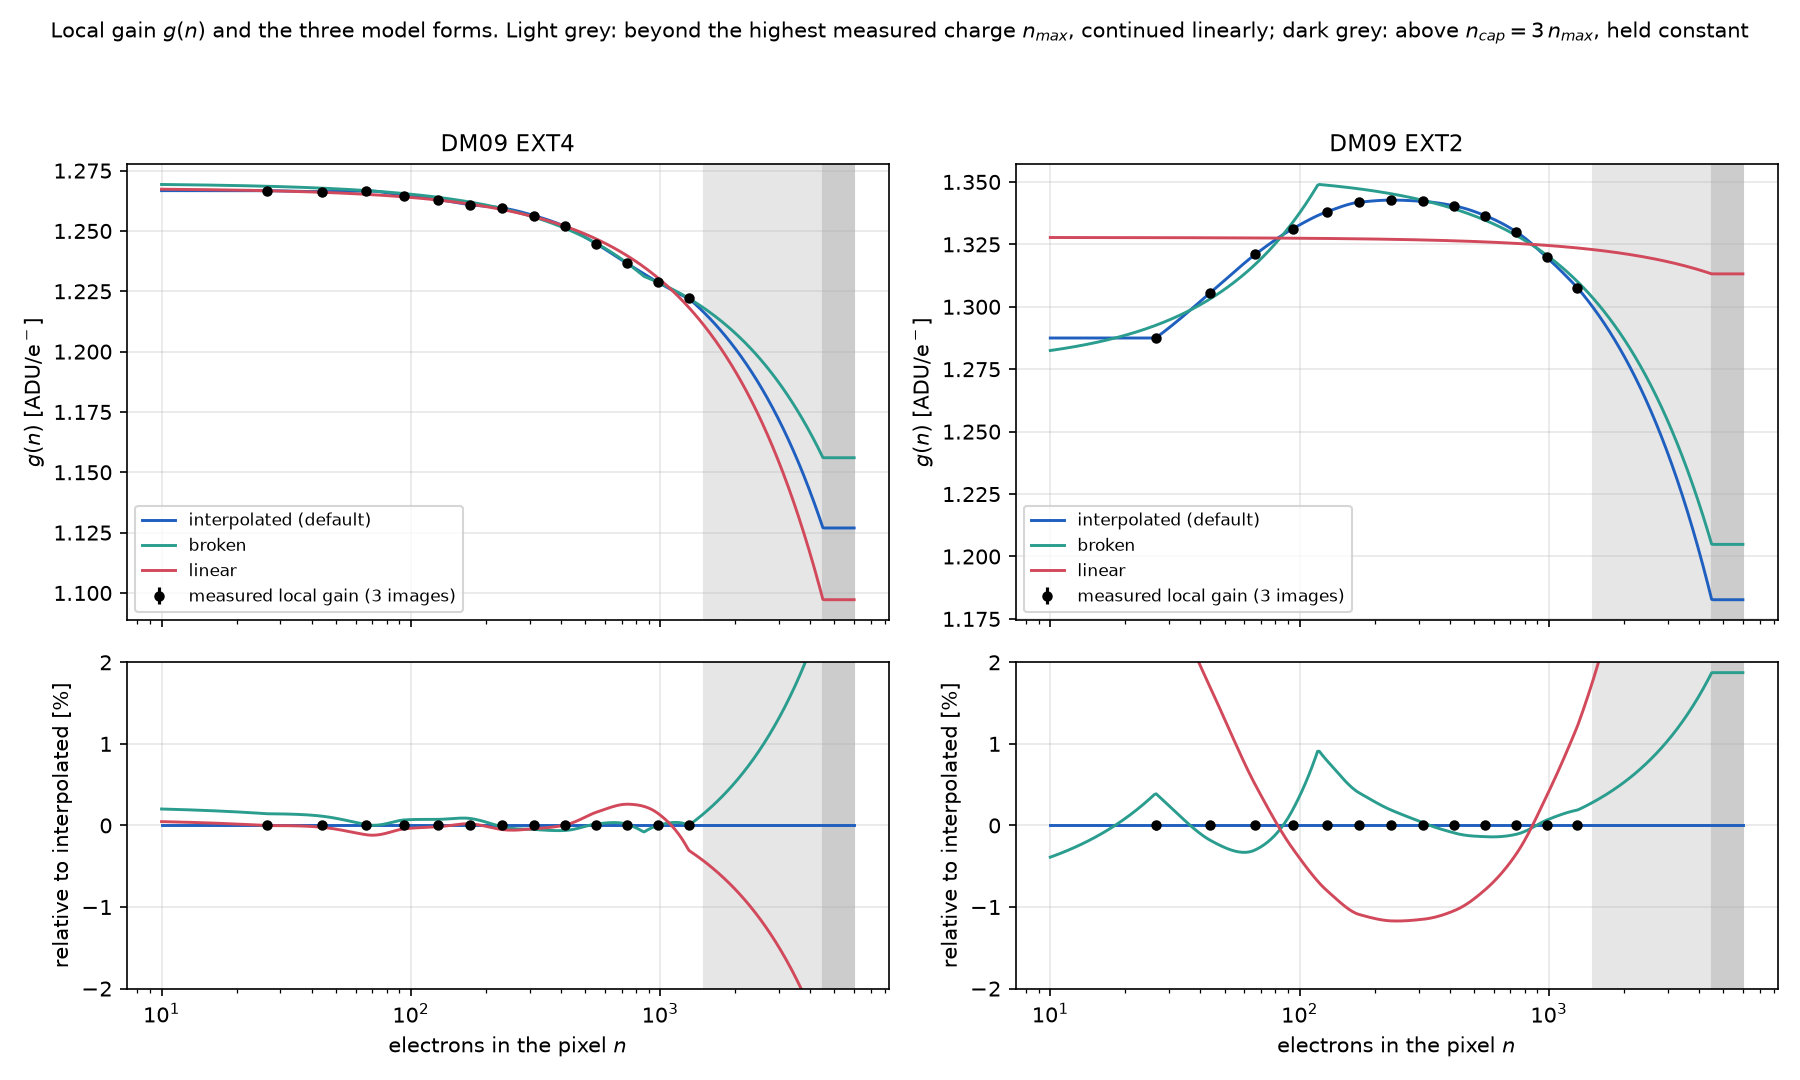
\includegraphics[width=\textwidth]{forms.png}
\caption{Measured local gain (points, 3 images) and the three model forms for two CCDs. EXT4 is the
usual case. On EXT2 the gain first \emph{rises} by $\sim$4\,\% from 25 to 200\,\eminus{} before it falls;
the interpolated and broken forms follow it, the straight line does not (it is off by up to 3\,\% at low
charge). Light grey: beyond $\nmax$ (continued linearly); dark grey: above $\ncap$ (constant). The forms
differ most there.}
\label{fig:forms}
\end{figure}

%======================================================================
\section{Applying the curve to cluster files}
%======================================================================
\code{gain\_vs\_charge.py apply} rewrites the pixel energies (\code{pixels\_E}) and cluster energies
(\code{Energy}) of panaSKImg cluster files. Everything else (positions, widths \code{fSTD\_X/Y}, pixel
lists, \ldots) is copied unchanged, so all cuts and the Fe-55 macro work as before.

\paragraph{Step 1: back to ADU.} The gain panaSKImg used is stored in the file
(\code{info} tree, \code{ext<N>\_gainext}), so Eq.~\ref{eq:epix} can be undone exactly:
\begin{equation}
x_j = \frac{E_{\mathrm{pix},j}}{\varepsilon}\,\gfit .
\end{equation}
\inwords{recover the pixel value in ADU that panaSKImg started from.}

\paragraph{Step 2: ADU to electrons.} Solve Eq.~\ref{eq:A} for the charge: $n_j = A^{-1}(x_j)$, the
number of electrons whose response is $x_j$. For the linear form this is the solution of the quadratic
equation $a\,n + \frac12 b\,n^2 = x$,
\begin{equation}
n = \frac{-a + \sqrt{a^2 + 2 b x}}{b} \quad (x \le A(\ncap)), \qquad
n = \ncap + \frac{x - A(\ncap)}{a + b\,\ncap} \quad (x > A(\ncap)),
\end{equation}
where the second expression covers the constant-gain region above $\ncap$. For the other forms $A(n)$ is
tabulated on a 1\,\eminus{} grid from 0 to $\ncap$ (trapezoid rule, as in Sec.~\ref{sec:deltapts}) and
inverted by linear interpolation in the table; above $\ncap$, $n = \ncap + (x - A(\ncap))/g(\ncap)$.
Negative pixel values (pure noise) are converted with $g(0)$.

\paragraph{Step 3: energies.} $E'_{\mathrm{pix},j} = \varepsilon\, n_j$ and $E' = \sum_j E'_{\mathrm{pix},j}$.

\begin{example}
DM09 EXT4, a pixel with 900 electrons. Its value is $x = A(900) = 1124.6$\,ADU. panaSKImg, with
$\gfit = 1.2759$, reports $E_{\mathrm{pix}} = 3.74\,\mathrm{eV} \times 1124.6/1.2759 = 3.296$\,keV, i.e.\
881 electrons. The correction recovers $x = 1124.6$\,ADU from 3.296\,keV and $\gfit$, then finds in the
table the charge with $A(n) = 1124.6$: $n = 900$, i.e.\ 3.366\,keV. For the six-pixel cluster of
Sec.~\ref{sec:bias} the energy goes from 5.813 back to 5.909\,keV.
\end{example}

\paragraph{The anchor.} By default (\code{--anchor comb}) the whole conversion uses the measured curve,
including its low-charge gain $g(0)$. This removes both terms of Eq.~\ref{eq:bias}, and all images of a
CCD are converted with the same curve, so image-to-image differences of $\gfit$ disappear. With
\code{--anchor fit} the image's own gain is kept at low charge: the pixel value is first scaled by
$g(0)/\gfit$, $x \to x\,g(0)/\gfit$, so that a low-charge pixel still gives $n = x/\gfit$ and only the
charge dependence is corrected (in the example above: 893 instead of 900 electrons). On DM24--26 the
\code{fit} anchor overshot by 0.8\,\% because the per-image gain fits were off by 1--4\,\%; \code{comb}
is the default.

%======================================================================
\section{In \code{run\_WADERs}}
%======================================================================
\begin{center}
\begin{tabular}{p{4.3cm}p{6.7cm}p{4.2cm}}
\toprule
option & what it does & output \\
\midrule
\code{--gain-correction} (= \code{pooled}) & one curve per module (ACM) from all its images (Sec.~\ref{sec:multi}) & \code{root\_gaincorr/} \\
\code{--gain-correction per-image} & each image corrected with its own curve; a CCD whose own comb is not usable gets the module curve (noted in \code{summary.txt}) & \code{root\_gaincorr\_per\_image/} \\
\code{--gain-correction both} & both, and a comparison per image and CCD (curve, cluster energies, front-side Fe-55 K$\alpha$) & both, and \code{gain\_vs\_charge/per\_image\_vs\_pooled.csv} \\
\code{--gain-model} & \code{interpolated} (default), \code{broken}, \code{linear} & \\
\code{--gain-anchor} & \code{comb} (default) or \code{fit} & \\
\bottomrule
\end{tabular}
\end{center}
Curves and plots are written to \code{gain\_vs\_charge/}: for every curve (per module and, with
\code{per-image} or \code{both}, per image) the local gain \code{*\_gain\_vs\_charge.png} and the
nonlinearity curve \code{*\_nonlinearity.png} (Fig.~\ref{fig:nonlin}); \code{summary.txt} lists $g(0)$, the
drop at 1000\,\eminus, $\nmax$ and the quadratic coefficients for each CCD. With \code{--composite}, the
Fe-55 macro is run on the corrected files (with \code{both}: also on the per-image ones, in
\code{composite\_per\_image/}). Example: \code{run\_WADERs images.txt --gain-correction both --composite}
(give the input before the flag).

%======================================================================
\section{Results: Fe-55, front side}
\label{sec:fe55}
%======================================================================
\paragraph{Data.} DM09 (ACM 109) and DM10 (ACM 106), three Image 5 exposures each (2025-08-27/28,
500 skips), run with \code{run\_WADERs}. Only front-side clusters are used, selected as in
\code{MakeComposite\_Fe55\_Clusters\_Extensions.cc}: the cluster width
$\sigma_{xy} = \sqrt{(\sigma_x^2 + \sigma_y^2)/2} < 1$ pixel (front-side X-rays convert near the gates and
diffuse little) and $4.5 < E < 7$\,keV; 850--1090 clusters per CCD for the three images together.
Default interpolated model, curve measured from the three images.

\paragraph{How K$\alpha$ is measured.} The cluster energies $E_k$ in 4.5--7\,keV are fitted without
binning (maximum likelihood) with the probability density
\begin{equation}
p(E) = (1 - f_{bg})\Big[(1 - f_\beta)\,G(E; \mu, \sigma) + f_\beta\,G\big(E; \tfrac{6.490}{5.899}\mu, \sigma\big)\Big]
+ \frac{f_{bg}}{2.5\ \mathrm{keV}},
\end{equation}
\inwords{a Gaussian $G$ for K$\alpha$ at $\mu$, a Gaussian of the same width for K$\beta$ at the energy
ratio of the two lines, and a flat background, with the fractions $f_\beta$ and $f_{bg}$ free.} The
parameters maximise $\prod_k p(E_k)$; the error of $\mu$ comes from the curvature of $-\ln L$.

\begin{table}[h]
\centering
\begin{tabular}{lrrrrr}
\toprule
CCD & clusters & without & interpolated & broken & linear \\
\midrule
DM09 EXT1 & 911 & 5.7308 & 5.8682 & 5.8679 & 5.8651 \\
DM09 EXT2 & 848 & 5.8221 & 5.8515 & 5.8489 & 5.8537 \\
DM09 EXT3 & 997 & 5.7781 & 5.8801 & 5.8798 & 5.8779 \\
DM09 EXT4 & 1020 & 5.7905 & 5.8839 & 5.8824 & 5.8823 \\
DM10 EXT1 & 1081 & 5.8927 & 5.8550 & 5.8527 & 5.8552 \\
DM10 EXT2 & 1091 & 6.1596 & 5.8436 & 5.8455 & 5.8400 \\
DM10 EXT4 & 1044 & 5.8854 & 5.8425 & 5.8426 & 5.8441 \\
\midrule
mean / spread & & 5.866 / 131\,eV & 5.861 / 16\,eV & 5.860 / 15\,eV & 5.860 / 15\,eV \\
\bottomrule
\end{tabular}
\caption{Front-side K$\alpha$ [keV] of the three images together (statistical error 1.8--2.4\,eV;
true 5.899\,keV), without and with the correction in its three forms. ``Spread'' is the standard
deviation over the 7 CCDs. DM10 EXT3 has no reliable curve and is not listed.}
\label{tab:fe55}
\end{table}

\begin{figure}[t]
\centering
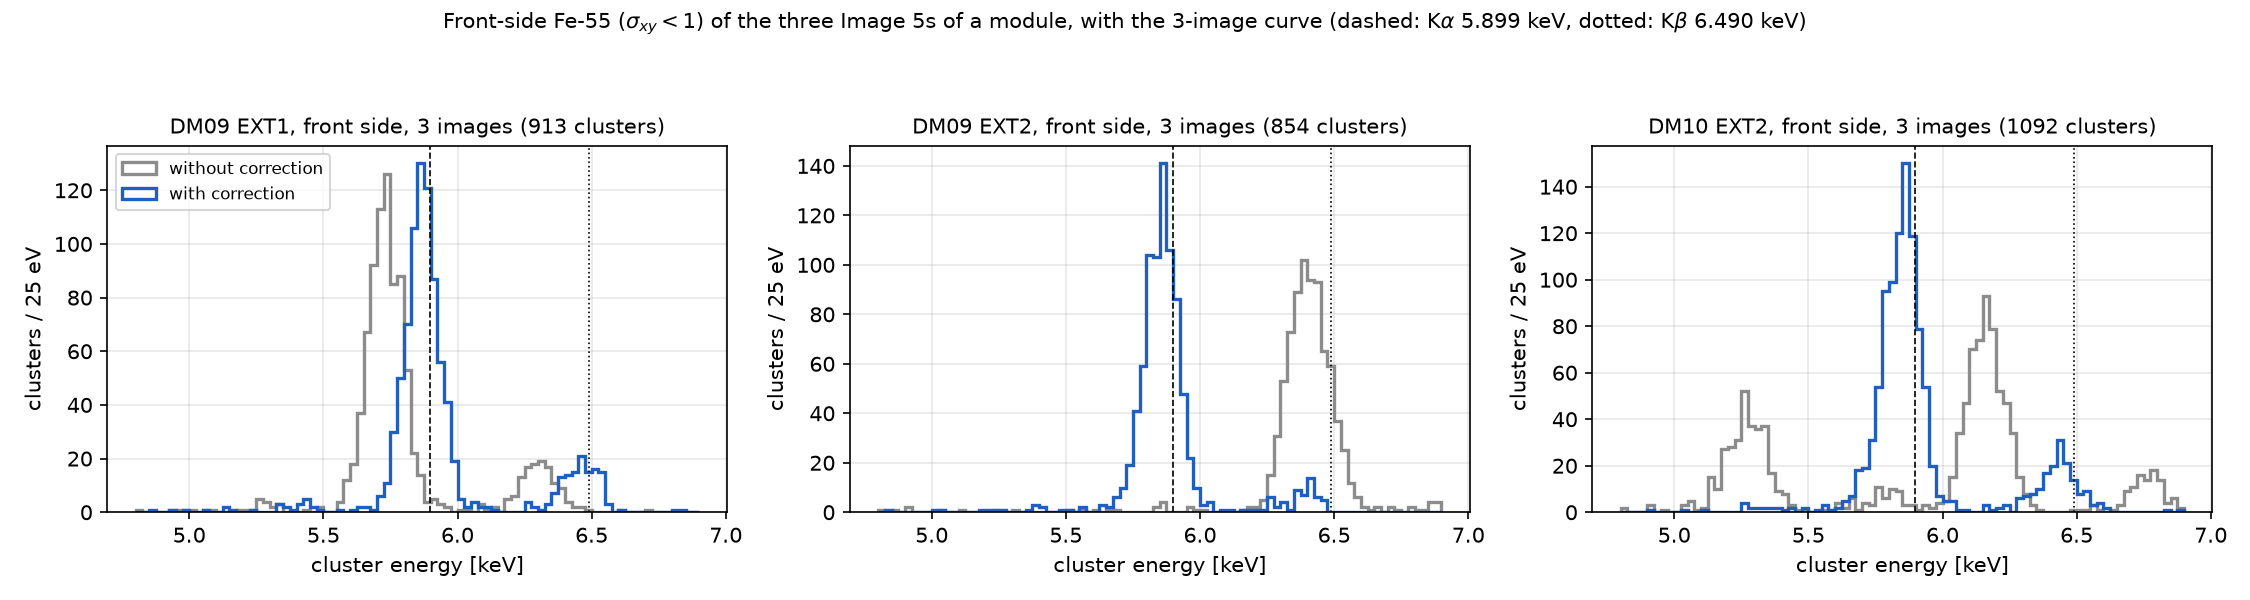
\includegraphics[width=\textwidth]{fe55.png}
\caption{Front-side Fe-55 spectra of the three Image 5s of a module, without and with the correction.
Without it the images of a CCD do not agree (two or three K$\alpha$ peaks on DM09 EXT2 and DM10 EXT2,
caused by the image-to-image differences of $\gfit$); with it there is one peak.}
\label{fig:fe55}
\end{figure}

\paragraph{What the correction does here.}
\begin{itemize}
\item The seven CCDs agree: spread 131\,eV $\to$ 16\,eV (Table~\ref{tab:fe55}, Fig.~\ref{fig:fe55}). Much
of the uncorrected scatter is the calibration term of Eq.~\ref{eq:bias}: $\gfit$ differs between the
images of a CCD (by 10--13\,\% on the noisy DM10 image 0 and $\sim$5\,\% on DM10 EXT2).
\item On DM09 EXT1, EXT3 and EXT4 the peaks move up by 90--140\,eV (1.6--2.4\,\%), the size that
Eq.~\ref{eq:bias} predicts for $\langle n\rangle_w \approx 1000$\,\eminus; on DM09 EXT2, whose gain first rises
(Fig.~\ref{fig:forms}), by 30\,eV. On DM10 EXT1 and EXT4 they move \emph{down} (e.g.\ 5.893
$\to$ 5.855\,keV): there $\gfit$ is $\sim$2\,\% below the low-charge gain of the comb (panaSKImg's gain
fits on DM10 have $\chi^2/\mathrm{ndf} \approx 30$), so term (i) of Eq.~\ref{eq:bias} happened to cancel
most of term (ii). After the correction DM10 agrees with DM09.
\item The corrected mean is 0.65\,\% below 5.899\,keV, the same for every curve and every model form, so it
is not a gain effect. The most likely cause is the charge in the faint edge of each cluster that
ClusterFinder's threshold drops; images with higher noise (and so a higher threshold) come out lower
(image 0 of DM09 and DM10, the noisier exposure: 5--60\,eV below images 1 and 2, with every curve).
\end{itemize}

\paragraph{One image or several?} The same front-side clusters were corrected with the curve of each
single image, of each pair and of all three. Relative to the 3-image curve, single-image curves change
K$\alpha$ by $-1.6$ to $+3.6$\,eV and 2-image curves by $-0.6$ to $+1.9$\,eV, against a statistical error of
2.1\,eV. Because the clusters are the same in every case, these differences come from the curves alone.
Per image, using another image's curve instead of its own changes K$\alpha$ by at most $\pm 5$\,eV.
\emph{A single Image 5 measures the curve well enough}; extra images add nothing measurable, except that
they provide a curve for an image whose own comb is unusable (DM10 image 0). The per-image and pooled
modes of \code{run\_WADERs} agree to 0--4\,eV on these data.

\paragraph{Earlier tests (linear model, previous code).} On 16 datasets (Images 5, 6, 7, 8, windowed and
1-skip readouts) the corrected front-side K$\alpha$ of 82 Image-5 CCDs went from 0.9835 to 0.9977 of the
true energy, with the CCD-to-CCD spread from 2.1\,\% to 0.32\,\% (about 20\,\% of CCDs had no reliable
curve; 1-skip images are correctly left alone). Images 6/7: 0.98--0.99 $\to$ 0.998--1.002. DM24--26
(2025-09-13): $5.831 \pm 0.131 \to 5.857 \pm 0.034$\,keV over 11 CCDs (mean $\pm$ spread). Details:
\code{docs/gain\_correction\_report.pdf}.

%======================================================================
\section{Results: Am-241}
\label{sec:am}
%======================================================================
\paragraph{Data.} AMTEst: 10 Image 8s (500 skips, board 106; EXT2 is flooded), all clusters. The comb
was measured once from the 10 images (Eq.~\ref{eq:Rmulti}) and the three forms were fitted to the same
points. Each line position is a binned fit of a Gaussian plus a linear background around the peak
(error scaled by $\sqrt{\chi^2/\mathrm{ndf}}$ when that is above 1).

\begin{table}[h]
\centering
\begin{tabular}{llrrrr}
\toprule
CCD & line & without & interpolated & broken & linear \\
\midrule
EXT3 & $\gamma$ 59.54\,keV & 0.9756 & 0.9981 & 0.9981 & 0.9975 \\
EXT4 & $\gamma$ 59.54\,keV & 0.9404 & 0.9932 & 0.9867 & 0.9944 \\
EXT4 & $\gamma$ 26.34\,keV & 0.9404 & 0.9898 & 0.9861 & 0.9903 \\
EXT4 & Np L$\beta$ 17.75\,keV & 0.9417 & 0.9844 & 0.9828 & 0.9823 \\
\bottomrule
\end{tabular}
\caption{Fitted line position divided by the true energy. Other lines (and EXT1) have no clear peak in
these partly flooded CCDs.}
\label{tab:am}
\end{table}

\begin{figure}[t]
\centering
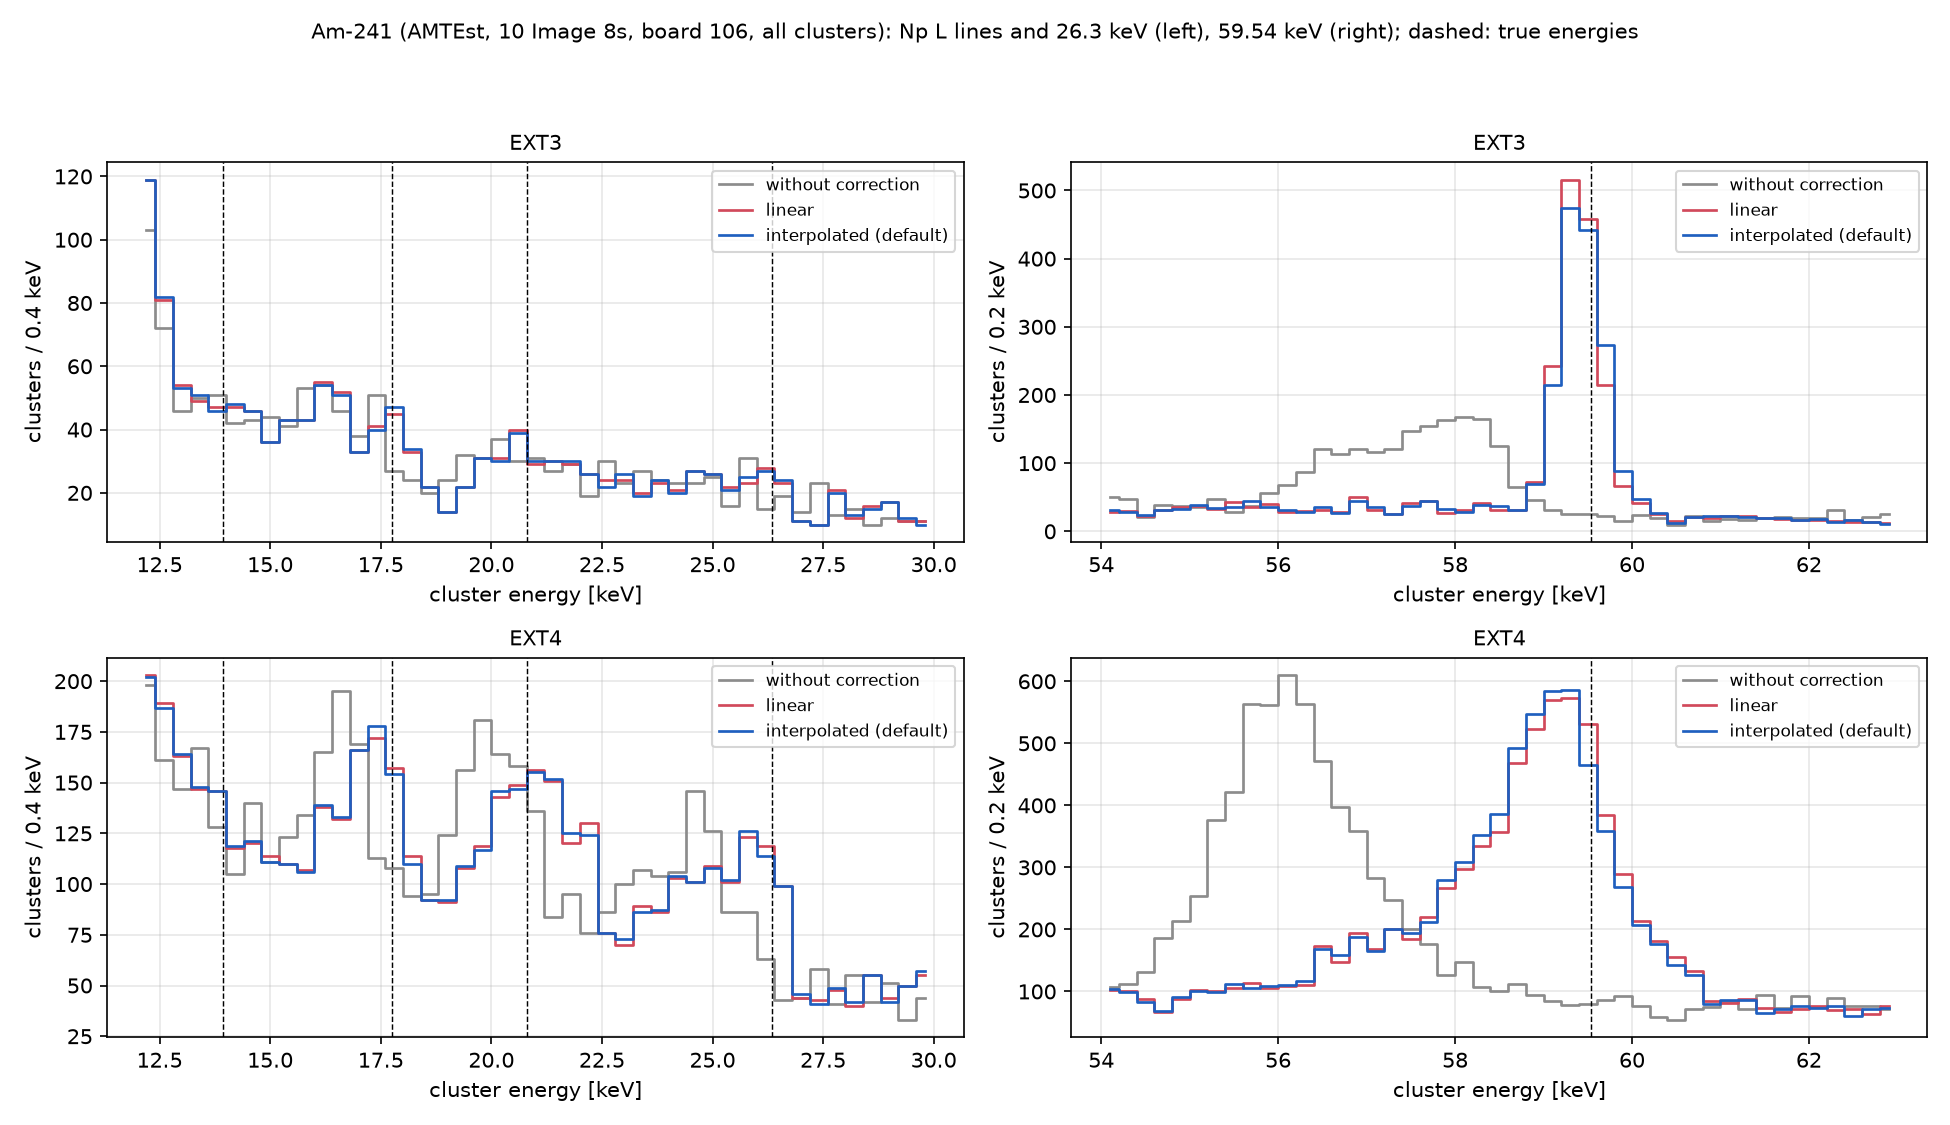
\includegraphics[width=\textwidth]{am241.png}
\caption{Am-241 spectra without correction and with the linear and interpolated curves.}
\label{fig:am}
\end{figure}

\paragraph{What it shows.} The correction moves the 59.5\,keV line from 2.4--6\,\% low to within
0.2--0.7\,\% with the default form (Table~\ref{tab:am}, Fig.~\ref{fig:am}). Here the model form matters more
than for Fe-55: the brightest pixel of a 59.5\,keV cluster typically holds 2400--2700\,\eminus{} (90\,\%
below $\sim$4500\,\eminus), while the comb is measured only up to $\nmax$ = 1130 (EXT3) and 850\,\eminus{}
(EXT4). Most of the correction therefore comes from the extrapolation between $\nmax$ and $\ncap$ and from
the constant gain above, and on EXT4 the forms differ by 0.8\,\% at 59.5\,keV. These numbers test the
extrapolation rule more than the measured curve, and the rule itself was tuned on this data set with the
linear form, so they are not an independent test of the forms.

%======================================================================
\section{Discussion: which model form?}
%======================================================================
The forms are judged by three questions.
\begin{itemize}
\item \textbf{Do they describe the measured points?} The quality of a description is measured by
$\chi^2/\mathrm{ndf} = \frac{1}{N_{pts} - N_{par}}\sum_k (g(n_k) - \hat g_k)^2/\sigma_k^2$; a value near 1 means
the curve passes the points within their errors. A straight line gives $\chi^2/\mathrm{ndf} > 30$ on every
CCD of the 2025-08-27 Image 5s, with the same curvature in every image of a CCD, so the curvature is a
property of the amplifier and not noise. The broken line and the interpolation follow the points. In a
separate scratch study with \emph{error-weighted} fits to each image's points (9 images, 36 CCD curves)
the median $\chi^2/\mathrm{ndf}$ of a curve on the \emph{other} images of the same CCD (a test that cannot be
passed by fitting noise) was 34 (straight line), 8.3 (quadratic), 5.6 (power law $a(1 - c\,n^p)$), 4.3 (broken
line), 2.6 (interpolation) and 136 ($a + c\ln n$). Fitted only up to 640\,\eminus{} and used to predict the
points at 850--1500\,\eminus, the rms error was 1.1, 1.3, 0.65, 0.50, 0.55 and 0.64\,\%.
\item \textbf{Do they change Fe-55 energies?} No (Table~\ref{tab:fe55}: within 4\,eV). The brightest pixels
of front-side Fe-55 clusters (median 1250\,\eminus, 90\,\% below 1520) are inside or just above the measured
range, where the integrals $A(n)$ of the three forms are still close; the forms separate only above
$\sim$2000\,\eminus{} (Fig.~\ref{fig:forms}). (The scratch study's error-weighted straight line spread the
CCDs more, 20 vs 11\,eV; the unweighted straight line used in the code does not.)
\item \textbf{Do they change higher energies?} Yes: Am-241 and tracks depend on the curve above $\nmax$,
i.e.\ on the extrapolation, where no form is measured.
\end{itemize}
The interpolated form is the default because it uses the measurement as it is, without imposing a shape,
and handles CCDs like DM09 EXT2 whose gain is not monotonic. The linear form is kept for comparison with
earlier results; the broken line is a compact alternative with similar behaviour.

%======================================================================
\section{Limitations and open points}
%======================================================================
\begin{itemize}
\item The remaining $-0.2$ to $-0.7$\,\% (Fe-55, Am-241) is not a gain effect; most likely cluster-edge charge
below the ClusterFinder threshold, larger for noisier images.
\item The comb is measured to 1000--1500\,\eminus; above, the curve is an assumption (linear to $3\,\nmax$,
then constant). A wider-range measurement (narrower charge bins at high charge, or a period allowed to
change within the bin) would remove most of this uncertainty.
\item Below the first point ($\approx 25$\,\eminus) nothing is measured and $g$ is held constant. On CCDs whose
gain rises at low charge (DM09 EXT2: panaSKImg's 0/1\,\eminus{} gain 1.22, comb 1.29 at 25\,\eminus{} and
1.34 at 200\,\eminus) the meaning of ``low-charge gain'' depends on the charge it refers to.
\item CCDs without a usable comb (noisy images, very low charge) get no curve of their own; with several
images of a module the module curve is used. Gains that rise with charge (DM10 EXT3) are rejected by the
reliability rule; why that CCD behaves differently is not understood.
\item The curve changes between campaigns (operating point of the output stage, temperature); it should be
measured per run, which one Image 5 is enough for.
\item The correction also replaces $\gfit$ by the comb's low-charge gain (anchor \code{comb}); where panaSKImg's
gain fits are poor (e.g.\ DM10, $\chi^2/\mathrm{ndf} \approx 30$) this is the larger effect.
\end{itemize}

\appendix
\section{Commands and files}
\begin{verbatim}
# measure (any number of images of the same module) and apply
python src/gain_vs_charge.py measure IMAGES... -o OUT --name NAME [--model interpolated|broken|linear]
python src/gain_vs_charge.py apply OUT/NAME_gain_vs_charge.json root/*_ext*.root -o root_gaincorr
# in the pipeline
run_WADERs images.txt --gain-correction [pooled|per-image|both] [--gain-model ...] [--composite]
\end{verbatim}
\code{measure} writes \code{NAME\_gain\_vs\_charge.json}, \code{NAME\_gain\_vs\_charge.png} and
\code{NAME\_nonlinearity.png}. The JSON holds, per extension: \code{points} (each bin: \code{n}, \code{n\_lo},
\code{n\_hi}, \code{g}, \code{err}, \code{visibility}, \code{npix}, \code{significant}), \code{model} (\code{form}
and its parameters; \code{a} is $g(0)$; \code{n\_cap}), \code{linear} (the straight-line fit used by the
reliability rule), \code{n\_max\_measured}, \code{drop\_at\_1000} $= 1 - g(1000)/g(0)$, \code{nonlinearity}
(\code{g\_ref} $= g(0)$, the points \code{n\_meas}, \code{delta}, \code{delta\_err}, the quadratic \code{c2},
\code{c1}, and \code{delta\_at\_1000} $= A(1000)/g(0) - 1000$), \code{g\_1e} ($g_0$),
\code{clean\_rows}/\code{rows}, \code{ok}/\code{reason}, and in per-image mode \code{source} (\code{image} or
\code{module}). The figures of this note are made by \code{make\_figures.py} (Am-241 numbers:
\code{am241\_forms.py}), in the same folder as this file.

\end{document}
